\documentclass{beamer}

\usepackage[linguistics]{forest}
\usepackage[utf8]{inputenc} 
\usepackage[T1]{fontenc}
\usepackage[croatian]{babel}
\usepackage{lmodern}

\usetheme{metropolis}
\title{Rješavanje problema rubikove kocke evolucijskim algoritmima}
\date{\today}
\author[Vinko Kolobara]{Vinko Kolobara\\{\small Mentor: prof.dr.sc Domagoj Jakobović}}
\institute{Fakultet elektrotehnike i računarstva, Zagreb, Hrvatska}


\begin{document}
  \maketitle
  
  \begin{frame}{Sadržaj}
  \setbeamertemplate{section in toc}[sections numbered]
  \tableofcontents
\end{frame}
  
  \section{Rubikova kocka}
  \begin{frame}{Problem rubikove kocke}
    \begin{columns}[T,onlytextwidth]
    	\column{0.5\textwidth}
		\begin{itemize}[<+- | alert@+>]
			\item općenito dimenzija $N\times N \times N$
			\item nizom dopuštenih poteza iz početnog stanja doći do ciljnog stanja
			\item velik broj stanja ($43 \times 10^{18}$)
			\item poznat božiji broj - 20
		\end{itemize}	
			    	    	
    	\column{0.5\textwidth}
    	\begin{figure}[h]
			\centering
			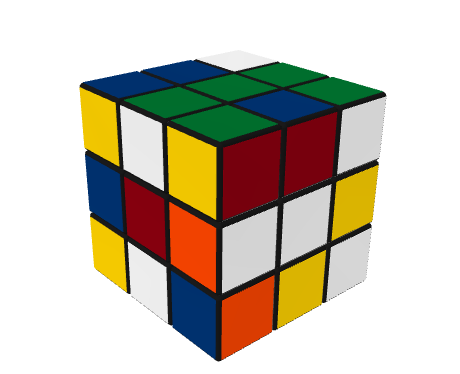
\includegraphics[width=0.45\textwidth]{../image/rubik_cube_scrambled.png}
			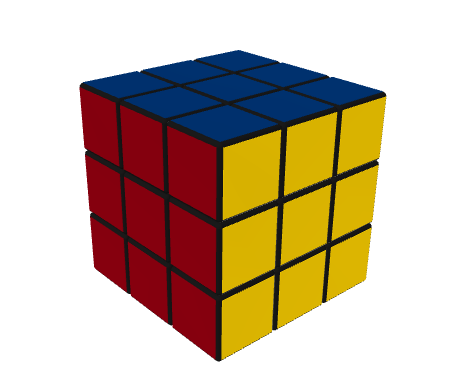
\includegraphics[width=0.45\textwidth]{../image/rubik_cube_solved.png}
			\caption{Primjer nekog nasumičnog početnog stanja rubikove kocke (lijeva slika) i prikaz ciljnog stanja (desna slika) }
		\end{figure}
    	
    \end{columns}
  \end{frame}
    
  \begin{frame}{Standardni algoritmi}
	\begin{itemize}[<+- | alert@+>]
		\item temeljeni na teoriji grupa
		\item Thistlewaite, Kociemba, Korf
	\end{itemize}
  \end{frame}

  \section{Evolucijski algoritmi i primjena na problem rubikove kocke}

  \begin{frame}{Ideja}
	\begin{itemize}[<+- | alert@+>]
		\item prevelik broj stanja za brute force
		\item evolucijski algoritmi dobri za kombinatorne probleme
		\item bez korištenja teorije grupa
	\end{itemize}
  \end{frame} 
  
  \subsection{Genetski algoritam}
  
  \begin{frame}{Genetski algoritam}
	\begin{figure}
		\centering
		\begin{tabular}{|c|c|c|c|c|}\hline
		2 & 0 & \dots & 7 & 15\\\hline
		\end{tabular}
		\caption{Primjer rješenja genetskog algoritma}
	\end{figure}  
  
	\begin{itemize}[<+- | alert@+>]
		\item genotip jedinke (niz poteza do rješenja)
		\item populacija jedinki
		\item genetski operatori (selekcija, križanje, \textbf{mutacija})
		\item mjera sposobnosti (fitness)
	\end{itemize}
  \end{frame}    
  
  \begin{frame}{Mjera sposobnosti}
	\begin{itemize}[<+- | alert@+>]
		\item zbroj ispravno pozicioniranih boja
		\item{ zbroj ispravno pozicioniranih rubnih i kutnih kockica + prethodna mjera 
	  	\begin{figure}[h]
		\centering
		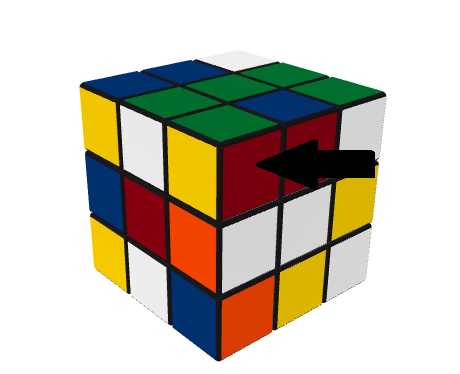
\includegraphics[width=0.45\textwidth]{../image/corner_cubie.png}
		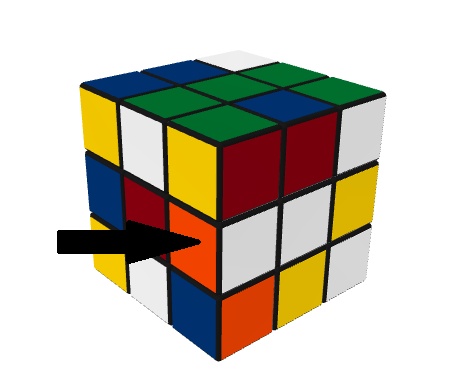
\includegraphics[width=0.45\textwidth]{../image/edge_cubie.png}
		\caption{Primjer kutne (lijeva slika) i rubne kockice (desna slika) }
  		\end{figure} }
  	\end{itemize}
  \end{frame}

  \subsection{Genetsko programiranje}
  
  \begin{frame}{Genetsko programiranje}
  	\begin{itemize}[<+- | alert@+>]
		\item genotip jedinke (stablo)
		\item populacija jedinki
		\item genetski operatori (selekcija, križanje, mutacija)
		\item mjera sposobnosti (fitness)
	\end{itemize}
  \end{frame}
  
  \begin{frame}{Genetsko programiranje - genotip}
    \begin{figure}[h]
	\centering
	\begin{forest}
  	[IfEdgeCubieCorrect(0)
    [IfCornerCubieCorrect(5)
    	[\textit{1}]
    	[\textit{11}]
    ]
    [\textit{15}]
  	]
	\end{forest}
	\caption{Primjer jednog dobivenog rješenja genetskim programiranjem}
	\end{figure}

  	\begin{itemize}[<+- | alert@+>]
		\item funkcijski čvorovi (IfEdgeCubieCorrect, IfCornerCubieCorrect)
		\item završni čvorovi (broj iz intervala $[0, 17]$)
	\end{itemize}	
	
  \end{frame}
  
  \section{Rezultati}
  
  \begin{frame}{Genetski algoritam}
  	\begin{itemize}[<+- | alert@+>]
		\item selekcija
		\item križanje
		\item mutacije
		\item parametri?
	\end{itemize}
  \end{frame}
  
  \begin{frame}{Genetski algoritam - prva mjera sposobnosti}
  		\begin{figure}[h]
			\centering
			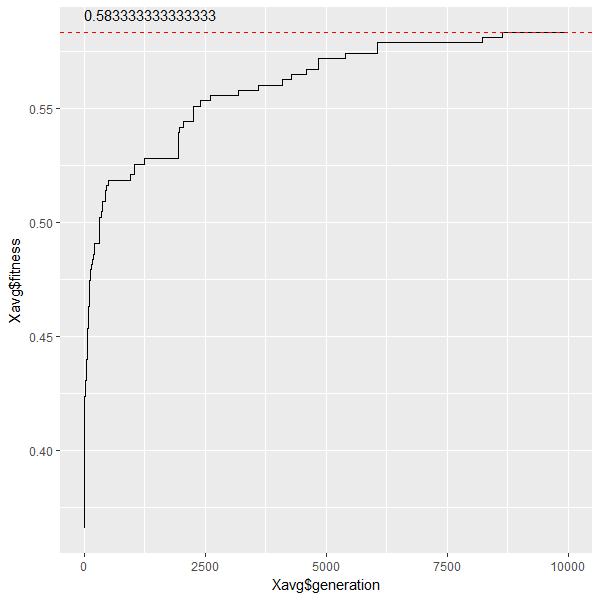
\includegraphics[width=0.5\textwidth]{../../results/sumsides_fitness/50_scrambles/cross0,5greedy10mut20.png}
			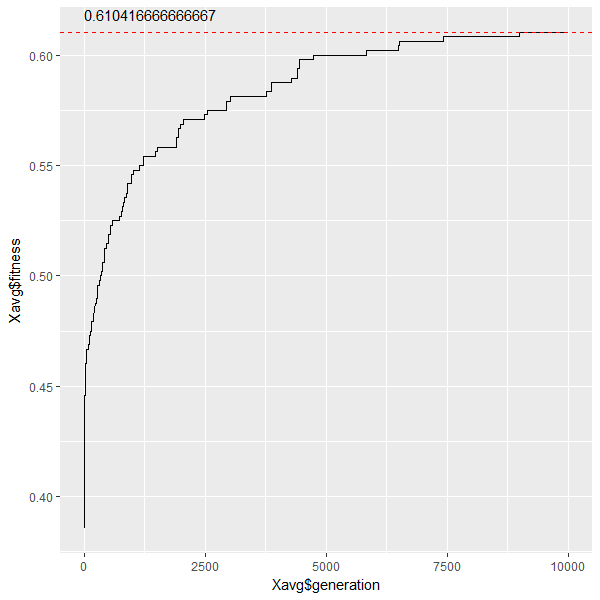
\includegraphics[width=0.5\textwidth]{../../results/sumsides_fitness/20_scrambles/cross0,5greedy10mut20.png}
			\caption{Prosječna vrijednost mjere sposobnosti po generacijama za 50 (lijevo) i 20 (desno) miješanja kocke }
		\end{figure}
  \end{frame}

  \begin{frame}{Genetski algoritam - prva mjera sposobnosti}
  		\begin{figure}[h]
			\centering
			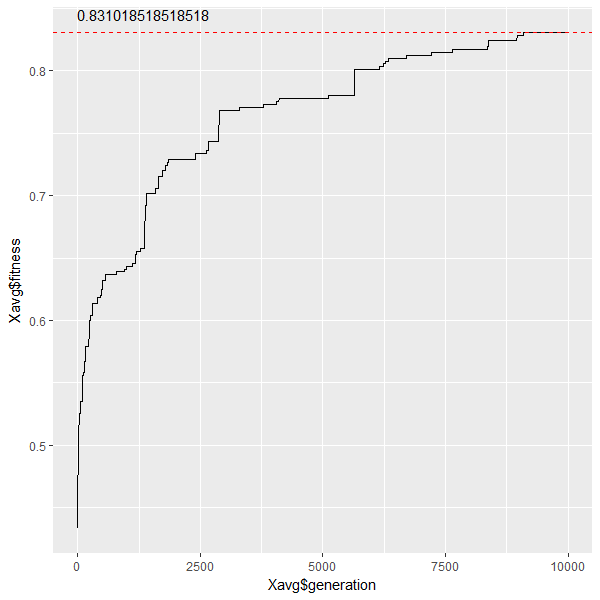
\includegraphics[width=0.5\textwidth]{../../results/sumsides_fitness/10_scrambles/cross0,5greedy10mut20.png}
			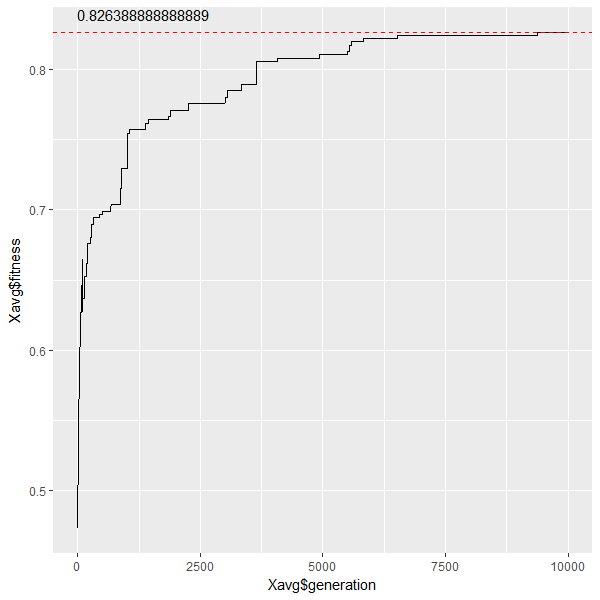
\includegraphics[width=0.5\textwidth]{../../results/sumsides_fitness/7_scrambles/cross0,5greedy10mut20.png}
			\caption{Prosječna vrijednost mjere sposobnosti po generacijama za 10 (lijevo) i 7 (desno) miješanja kocke }
		\end{figure}
  \end{frame}  
    
  \begin{frame}{Genetski algoritam - prva mjera sposobnosti}
  		\begin{figure}[h]
			\centering
			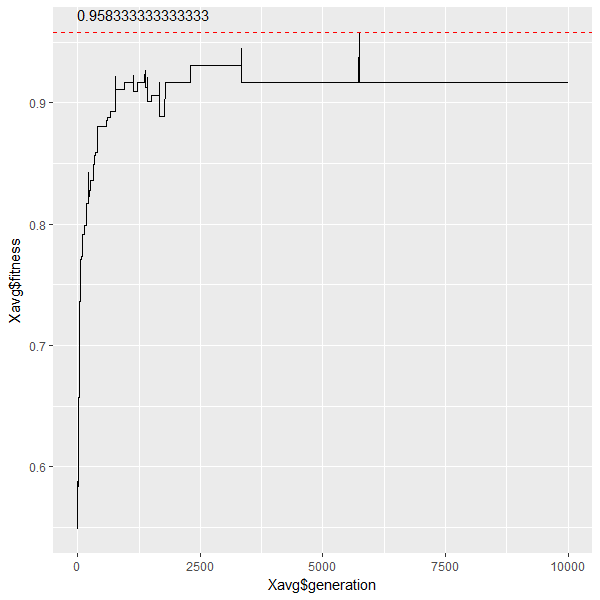
\includegraphics[width=0.6\textwidth]{../../results/sumsides_fitness/5_scrambles/cross0,5greedy10mut20.png}
			\caption{Prosječna vrijednost mjere sposobnosti po generacijama za 5 miješanja kocke }
		\end{figure}
  \end{frame}  
    
  \begin{frame}{Genetski algoritam - druga mjera sposobnosti}
  		\begin{figure}[h]
			\centering
			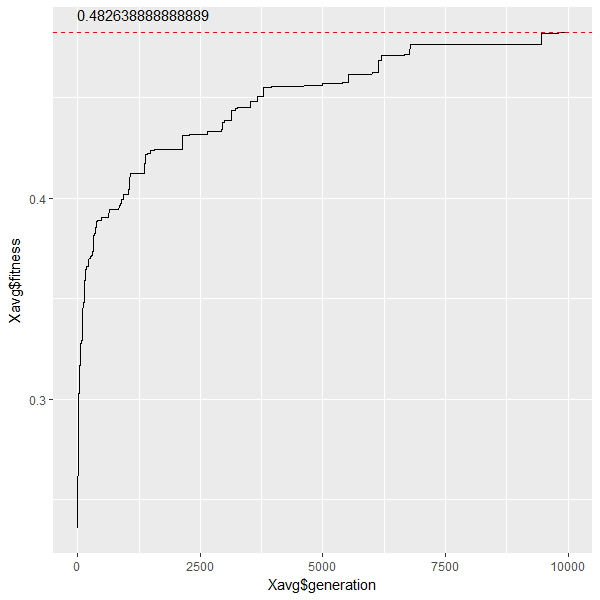
\includegraphics[width=0.5\textwidth]{../../results/cubies_fitness/50_scrambles/cross0,5greedy10mut20.png}
			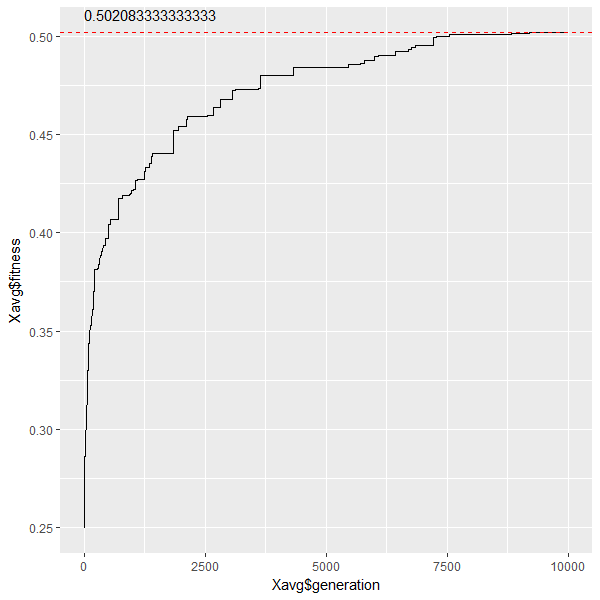
\includegraphics[width=0.5\textwidth]{../../results/cubies_fitness/20_scrambles/cross0,5greedy10mut20.png}
			\caption{Prosječna vrijednost mjere sposobnosti po generacijama za 50 (lijevo) i 20 (desno) miješanja kocke }
		\end{figure}
  \end{frame}

  \begin{frame}{Genetski algoritam - druga mjera sposobnosti}
  		\begin{figure}[h]
			\centering
			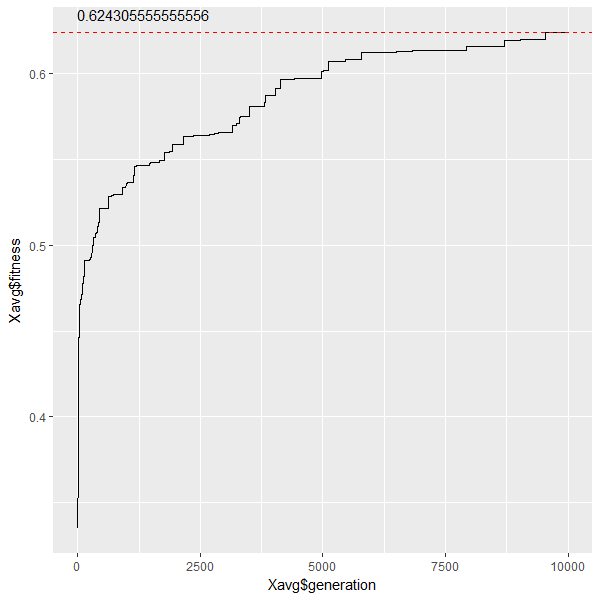
\includegraphics[width=0.5\textwidth]{../../results/cubies_fitness/10_scrambles/cross0,5greedy10mut20.png}
			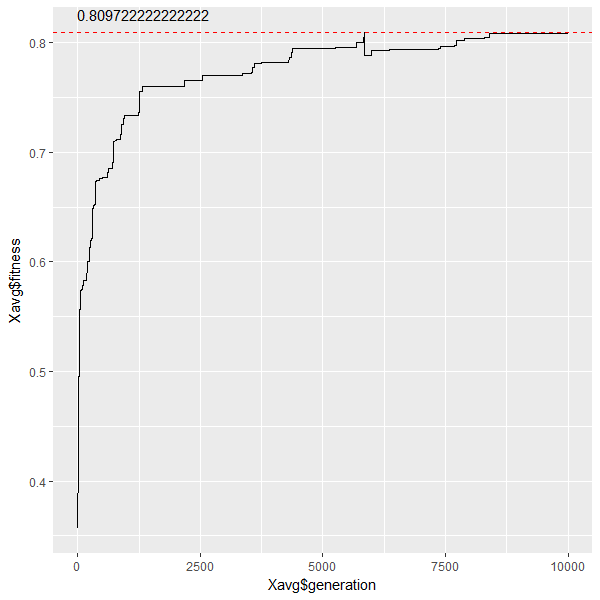
\includegraphics[width=0.5\textwidth]{../../results/cubies_fitness/7_scrambles/cross0,5greedy10mut20.png}
			\caption{Prosječna vrijednost mjere sposobnosti po generacijama za 10 (lijevo) i 7 (desno) miješanja kocke }
		\end{figure}
  \end{frame}  
    
  \begin{frame}{Genetski algoritam - druga mjera sposobnosti}
  		\begin{figure}[h]
			\centering
			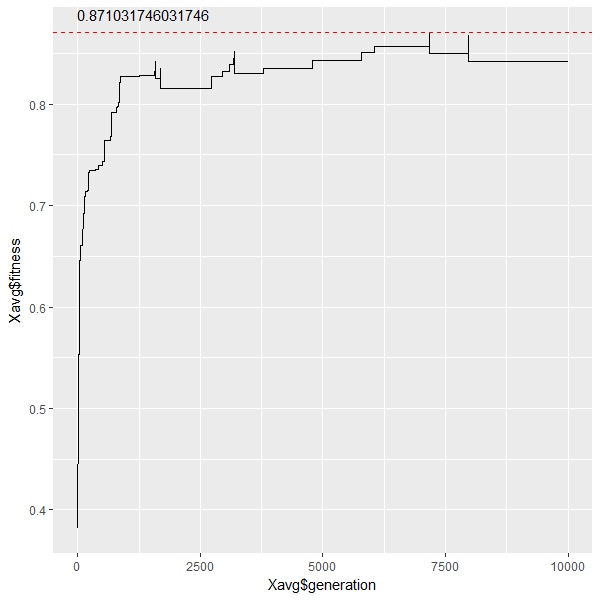
\includegraphics[width=0.6\textwidth]{../../results/cubies_fitness/5_scrambles/cross0,5greedy10mut20.png}
			\caption{Prosječna vrijednost mjere sposobnosti po generacijama za 5 miješanja kocke }
		\end{figure}
  \end{frame}
  
  \begin{frame}{Demonstracija}
  \end{frame}
    
\end{document}